\documentclass{BeamerTemplate}

\usepgfplotslibrary{statistics}

\title{Chapitre 4 -- Comparaison de deux populations}
\subtitle{STT-1920 Méthodes statistiques}
\date{}

\pgfplotsset{
  base/.style={
    tick label style={font=\scriptsize}, label style={font=\small},
    title style={font=\small\bfseries},
    yticklabel style={/pgf/number format/fixed, /pgf/number format/precision=2},
    scaled y ticks=false,
  },
  % Style des courbes de densité avec zones de rejet
  densite/.style={
    base, width=11cm, height=4.8cm,
    axis lines=left, ymin=0, ytick=\empty,
    xlabel style={font=\small}, clip=false,
  },
  % Style des diagrammes en boîtes juxtaposés
  boites/.style={
    base, width=5.6cm, height=5cm,
    boxplot/draw direction=y,
    axis lines=left, ymajorgrids, grid style={black!10},
    xtick={1,2}, xmin=0.4, xmax=2.6,
  },
}

% Densités utilisées pour les zones de rejet
\tikzset{declare function={
  fF(\x) = 34.02*\x*\x*(1+1.2*\x)^(-5.5);   % densité F(6, 5)
  ft(\x) = 0.38999*(1+\x*\x/11)^(-6);        % densité t à 11 d.l.
  fz(\x) = exp(-\x*\x/2)/sqrt(2*pi);         % densité N(0, 1)
}}

% Couleurs des deux groupes
\colorlet{grUn}{Dominante!85!black}
\colorlet{grDeux}{Accent}

% Arbre de décision : quel test utiliser ?
\tikzset{
  arbreQ/.style={draw=Dominante!80!black, fill=Dominante!20, rounded corners=2pt,
                 align=center, inner sep=3pt, text width=#1},
  arbreQ/.default=2.6cm,
  arbreR/.style={draw=Accent, fill=Accent!15, rounded corners=2pt,
                 align=center, inner sep=3pt, text width=#1},
  arbreR/.default=2.6cm,
  arbreFl/.style={-{Stealth[length=2mm]}, thick, black!60},
  arbreLab/.style={font=\scriptsize\itshape, fill=Fond, inner sep=1pt},
}
\newcommand{\ArbreDecision}{%
  \begin{tikzpicture}[font=\footnotesize]
    \node[arbreQ=4.6cm] (depart) at (0,0) {\textbf{Que veut-on comparer ?}};
    \node[arbreQ=3.6cm] (var)  at (-4.9,-1.25) {Deux \textbf{variances}\\(dispersion)};
    \node[arbreQ=3.6cm] (moy)  at (0,-1.25)    {Deux \textbf{moyennes}};
    \node[arbreQ=3.6cm] (prop) at (4.9,-1.25)  {Deux \textbf{proportions}\\(variable binaire)};
    \node[arbreR=3.6cm] (fisher) at (-4.9,-2.7) {\textbf{Test $F$ de Fisher}\\\texttt{var.test()}};
    \node[arbreR=3.6cm] (ztest)  at (4.9,-2.7)  {\textbf{Test $z$} ($\widehat{P}$ combinée)\\\texttt{prop.test()}};
    \node[arbreQ=3.6cm] (app) at (0,-2.7) {Données \textbf{appariées} ?};
    \node[arbreR=3.8cm] (tapp) at (-3.0,-4.2) {\textbf{Test $t$ apparié} sur les $D_i$\\\texttt{paired=TRUE}};
    \node[arbreQ=3.8cm] (testF) at (2.4,-4.2) {Indépendants : test $F$\\$H_0: \sigma_1^2 = \sigma_2^2$ ?};
    \node[arbreR=5cm] (pool) at (-0.6,-5.8) {\textbf{Test $t$ à variance combinée}\\\texttt{var.equal=TRUE}};
    \node[arbreR=3.8cm] (welch) at (4.9,-5.8) {\textbf{Test de Welch}\\\texttt{var.equal=FALSE}};
    \draw[arbreFl] (depart) -- (var);  \draw[arbreFl] (depart) -- (moy);  \draw[arbreFl] (depart) -- (prop);
    \draw[arbreFl] (var) -- (fisher);  \draw[arbreFl] (prop) -- (ztest);  \draw[arbreFl] (moy) -- (app);
    \draw[arbreFl] (app) -- node[arbreLab, pos=0.45] {oui} (tapp);
    \draw[arbreFl] (app) -- node[arbreLab, pos=0.45] {non} (testF);
    \draw[arbreFl] (testF) -- node[arbreLab, pos=0.4, left] {non rejetée} (pool);
    \draw[arbreFl] (testF) -- node[arbreLab, pos=0.4, right] {rejetée} (welch);
  \end{tikzpicture}%
}

\begin{document}

\begin{frame}[t]
  \titlepage
\end{frame}

%===============================================================================
\section{Introduction et objectifs}
%===============================================================================

\begin{frame}[t]{Où en sommes-nous ?}
  \textbf{Au chapitre 3c}, on a testé si \alert{un} paramètre prend une valeur précise :
  $H_0: \mu = 120$ mmHg, \ $H_0: p = 0{,}10$, etc.

  \medskip
  \textbf{Au chapitre 4}, on dispose de \alert{deux échantillons} et on veut savoir si le paramètre prend la \alert{même valeur dans deux populations} :
  \begin{itemize}\itemsep 1mm
    \item La concentration moyenne de zinc est-elle la même dans deux rivières ?
    \item Un antihypertenseur diminue-t-il la pression artérielle des patients ?
    \item Le taux de guérison d'un nouveau traitement dépasse-t-il celui du traitement standard ?
    \item La variabilité du poids des fruits est-elle la même dans deux vergers ?
  \end{itemize}

  \begin{Boite}{Rappel du chapitre 3c : les étapes d'un test}
    \small
    1) $H_0$ et $H_1$ ; \ 2) seuil $\alpha$ et loi de la statistique sous $H_0$ ; \ 3) statistique observée ; \ 4) décision (région critique ou valeur-p) ; \ 5) \alert{conclusion en mots}.
  \end{Boite}
\end{frame}

\begin{frame}[t]{Objectifs du chapitre}
  Dans de nombreuses applications réelles (agronomie, biologie, santé, écologie), on souhaite \alert{comparer deux traitements, deux groupes ou deux conditions expérimentales}.

  \medskip
  \begin{Boite}{Objectifs principaux}
    \begin{enumerate}\itemsep 2mm
      \item \textbf{Estimer} la différence ou le rapport de deux paramètres associés à deux populations ($\mu_1 - \mu_2$, $\sigma_1^2/\sigma_2^2$, $p_1 - p_2$).
      \item \textbf{Calculer} l'erreur-type associée et construire un \alert{intervalle de confiance}.
      \item \textbf{Tester} une hypothèse sur ces deux paramètres (ex. : $H_0: \mu_1 = \mu_2$ ou $H_0: \sigma_1^2 = \sigma_2^2$) à l'aide d'un \alert{test d'hypothèses}.
      \item \textbf{Choisir} le bon test selon le plan d'échantillonnage et \textbf{lire} une sortie R.
    \end{enumerate}
  \end{Boite}
\end{frame}

\begin{frame}[t]{Les 5 situations étudiées}
  \scriptsize
  \renewcommand{\arraystretch}{1.25}
  \begin{tabularx}{\textwidth}{llX}\toprule
    \textbf{Paramètres} & \textbf{Hypothèse} & \textbf{Conditions expérimentales} \\ \midrule
    \textbf{Deux variances} & $H_0: \sigma_1^2 = \sigma_2^2$ & Échantillons indépendants, populations normales \\ \midrule
    \multirow{3}{*}{\textbf{Deux moyennes}} & \multirow{3}{*}{$H_0: \mu_1 = \mu_2$}
      & 1. Indépendants, normales, \alert{$\sigma_1^2 = \sigma_2^2$} (variance combinée) \\
      & & 2. Indépendants, normales, \alert{$\sigma_1^2 \ne \sigma_2^2$} (Welch-Satterthwaite) \\
      & & 3. Échantillons \alert{appariés} (mesures dépendantes deux à deux) \\ \midrule
    \textbf{Deux proportions} & $H_0: p_1 = p_2$ & Indépendants, $n_1, n_2$ grands (approximation normale) \\ \bottomrule
  \end{tabularx}

  \bigskip
  \uncover<2->{
  \begin{Boite}{Ordre d'analyse logique pour deux moyennes}
    Lorsque les échantillons sont indépendants, on commence \alert{toujours} par tester l'égalité des variances ($\sigma_1^2$ vs $\sigma_2^2$) pour choisir le test de comparaison des moyennes approprié !
  \end{Boite}
  }
\end{frame}

\begin{frame}[t]{Feuille de route : quel test utiliser ?}
  \centering
  \ArbreDecision
\end{frame}

\begin{frame}[t]{Exemple 1 : Le zinc dans les rivières}
  On cherche à diversifier l'alimentation en eau potable d'une municipalité.
  \begin{itemize}\itemsep 1mm
    \item Deux rivières sont candidates, mais les biologistes soupçonnent que la \textbf{rivière 1} a une concentration moyenne en zinc supérieure à celle de la \textbf{rivière 2}.
    \item On suppose que les concentrations de zinc suivent des lois normales.
  \end{itemize}

  \medskip
  Mesures prélevées (en $\mu\text{g/l}$) à des sites choisis au hasard dans chaque rivière :

  \smallskip
  {\centering
  \small
  \begin{tabular}{lccccccccc}\toprule
    \textbf{Site} & 1 & 2 & 3 & 4 & 5 & 6 & 7 & $\bar{x}$ & $s$ \\ \midrule
    \textbf{Rivière 1} ($n_1 = 7$) & 6{,}51 & 5{,}43 & 4{,}32 & 5{,}73 & 3{,}90 & 4{,}11 & 5{,}00 & \textbf{5{,}00} & \textbf{0{,}954} \\
    \textbf{Rivière 2} ($n_2 = 6$) & 6{,}03 & 4{,}92 & 3{,}60 & 5{,}13 & 2{,}58 & 4{,}08 & -- & \textbf{4{,}39} & \textbf{1{,}226} \\ \bottomrule
  \end{tabular}
  \par}

  \medskip
  \uncover<2->{
    \textbf{Question 1 :} au seuil $\alpha = 10\%$, les variances sont-elles égales ? \\
    \textbf{Question 2 :} au seuil $\alpha = 5\%$, la rivière 1 contient-elle plus de zinc en moyenne ?
  }
\end{frame}

\begin{frame}[t]{Exemple 1 : Toujours regarder les données d'abord}
  \begin{columns}[T]
    \column{0.5\textwidth}
      \centering
      \begin{tikzpicture}
        \begin{axis}[boites, xticklabels={Rivière 1, Rivière 2},
                     ylabel={Zinc ($\mu$g/l)}, ymin=2, ymax=7]
          \addplot+[boxplot prepared={median=5.00, lower quartile=4.215,
              upper quartile=5.58, lower whisker=3.90, upper whisker=6.51},
              draw=grUn, fill=grUn!25, solid, mark=none] coordinates {};
          \addplot+[boxplot prepared={median=4.50, lower quartile=3.72,
              upper quartile=5.0775, lower whisker=2.58, upper whisker=6.03},
              draw=grDeux, fill=grDeux!25, solid, mark=none] coordinates {};
          \addplot[only marks, mark=*, mark size=1.3pt, black!70] coordinates {
            (1.25,6.51) (1.25,5.43) (1.25,4.32) (1.25,5.73) (1.25,3.90) (1.25,4.11) (1.25,5.00)
            (2.25,6.03) (2.25,4.92) (2.25,3.60) (2.25,5.13) (2.25,2.58) (2.25,4.08)};
        \end{axis}
      \end{tikzpicture}

    \column{0.48\textwidth}
      \small
      \begin{itemize}\itemsep 3mm
        \item Les \alert{diagrammes en boîtes juxtaposés} permettent de comparer d'un coup d'\oe il le \textbf{centre} et la \textbf{dispersion}.
        \item Ici : médianes proches, boîtes qui se chevauchent beaucoup ; dispersion un peu plus grande pour la rivière 2.
        \item Avec $n_1 = 7$ et $n_2 = 6$, difficile de conclure « à l'\oe il » : il faut un \alert{test}.
      \end{itemize}
  \end{columns}
\end{frame}

\begin{frame}[plain,t]
  \centerline{\LARGE\bfseries\alert{QUIZ !}}

  \medskip
  Dans l'exemple du zinc :
  \begin{itemize}\itemsep 0.7cm
    \item Les deux échantillons sont-ils indépendants ou appariés ?
    \item<2-> \alert{Indépendants} : sites différents dans deux rivières différentes, aucune correspondance naturelle entre le site 1 de la rivière 1 et le site 1 de la rivière 2 (d'ailleurs $n_1 \neq n_2$).
    \item Quelles hypothèses pour la question 2 ? Test unilatéral ou bilatéral ?
    \item<2-> $H_0: \mu_1 = \mu_2$ contre $H_1: \mu_1 > \mu_2$ : \alert{unilatéral à droite} (les biologistes soupçonnent une concentration \emph{supérieure} dans la rivière 1).
  \end{itemize}
\end{frame}

%===============================================================================
\section{Comparaison de deux variances (Test de Fisher)}
%===============================================================================

\begin{frame}[t]{Situation et distribution d'échantillonnage}
  Soient deux échantillons aléatoires indépendants :
  $$X_{11}, \ldots, X_{1n_1} \overset{iid}{\sim} \mathcal{N}(\mu_1, \sigma_1^2) \quad \text{et} \quad X_{21}, \ldots, X_{2n_2} \overset{iid}{\sim} \mathcal{N}(\mu_2, \sigma_2^2)$$

  \begin{itemize}\itemsep 3mm
    \item On sait que $\frac{(n_1-1)S_1^2}{\sigma_1^2} \sim \chi^2_{n_1-1}$ et $\frac{(n_2-1)S_2^2}{\sigma_2^2} \sim \chi^2_{n_2-1}$.
    \item Le rapport de deux v.a. khi-deux indépendantes divisées par leurs degrés de liberté respectifs suit une \alert{loi de Fisher-Snedecor}.
  \end{itemize}

  \bigskip
  \pause
  \begin{Boite}{Statistique fondamentale}
    \[
      F = \frac{S_1^2 / \sigma_1^2}{S_2^2 / \sigma_2^2} \sim \mathcal{F}(n_1-1,\, n_2-1)
    \]
  \end{Boite}
\end{frame}

\begin{frame}[t]{Propriétés de la loi de Fisher $\mathcal{F}(\nu_1, \nu_2)$}
  \begin{columns}[T]
    \column{0.5\textwidth}
      \begin{itemize}\itemsep 2mm
        \item Variable toujours \alert{strictement positive} ($F > 0$).
        \item Distribution \alert{asymétrique à droite}.
        \item Dépend de deux paramètres : $\nu_1$ degrés de liberté au numérateur, $\nu_2$ au dénominateur (\alert{l'ordre compte !}).
        \item Propriété d'inversion des quantiles :
          $$F_{1-\alpha,\, \nu_1,\, \nu_2} = \frac{1}{F_{\alpha,\, \nu_2,\, \nu_1}}$$
        \item Dans R : \texttt{qf(0.95, 6, 5)} donne $F_{0{,}05;\,6,\,5} = 4{,}95$.
      \end{itemize}

    \column{0.48\textwidth}
      \centering
      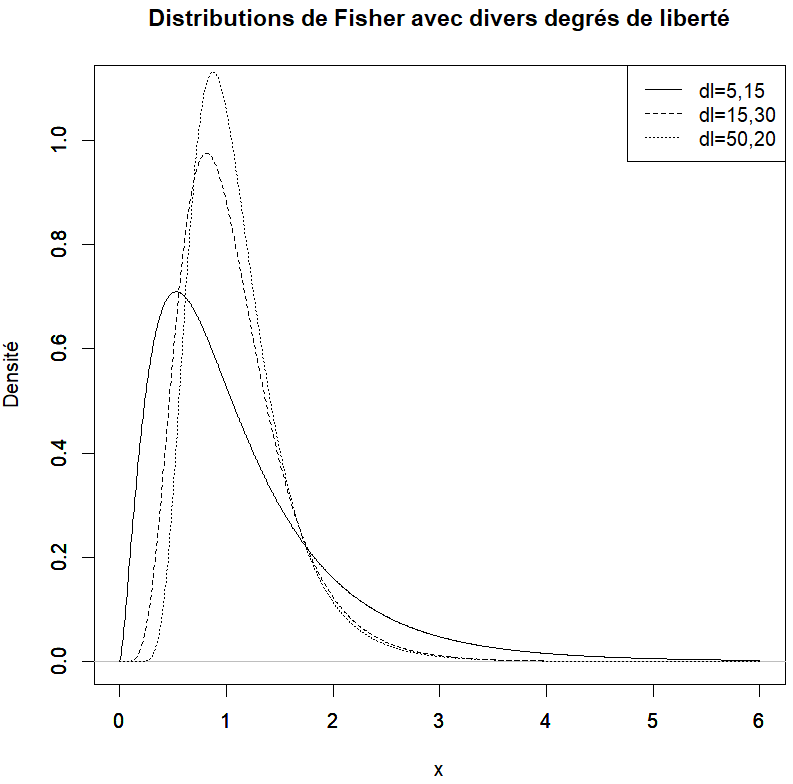
\includegraphics[width=\linewidth]{images/Fisher.PNG}
  \end{columns}
\end{frame}

\begin{frame}[t]{Intervalle de confiance pour $\sigma_1^2 / \sigma_2^2$}
  En partant de $P\left(F_{1-\alpha/2} \le \frac{S_1^2/\sigma_1^2}{S_2^2/\sigma_2^2} \le F_{\alpha/2}\right) = 1 - \alpha$, on isole le rapport $\frac{\sigma_1^2}{\sigma_2^2}$ :

  \bigskip
  \begin{Boite}{Intervalle de confiance à $1-\alpha$ pour $\sigma_1^2 / \sigma_2^2$}
    $$\left[ \frac{S_1^2}{S_2^2} \, \frac{1}{F_{\alpha/2,\, n_1-1,\, n_2-1}}, \quad \frac{S_1^2}{S_2^2} \, F_{\alpha/2,\, n_2-1,\, n_1-1} \right]$$
  \end{Boite}

  \bigskip
  \uncover<2->{
  \begin{itemize}\itemsep 3mm
    \item Attention à l'\alert{inversion des degrés de liberté} dans la borne supérieure !
    \item Si l'intervalle contient la valeur \textbf{1}, on ne peut pas rejeter l'hypothèse d'égalité des variances ($\sigma_1^2 = \sigma_2^2$).
  \end{itemize}
  }
\end{frame}

\begin{frame}[t]{Test de Fisher pour l'égalité des variances}
  \begin{itemize}\itemsep 1mm
    \item \textbf{Hypothèses :} $H_0: \sigma_1^2 = \sigma_2^2$ \quad contre \quad $H_1: \sigma_1^2 \ne \sigma_2^2$ (bilatéral)
    \item \textbf{Statistique de test sous $H_0$ :}
      $F_{obs} = s_1^2 / s_2^2$, à comparer à la loi $\mathcal{F}(n_1-1,\, n_2-1)$
    \item \textbf{Règle de décision au seuil $\alpha$ :}
      $$\text{Rejeter } H_0 \iff F_{obs} < \frac{1}{F_{\alpha/2,\, n_2-1,\, n_1-1}} \quad \text{ou} \quad F_{obs} > F_{\alpha/2,\, n_1-1,\, n_2-1}$$
    \item \textbf{Unilatéral} ($H_1: \sigma_1^2 > \sigma_2^2$) : rejeter $H_0$ si $F_{obs} > F_{\alpha,\, n_1-1,\, n_2-1}$.
    \item \textbf{Valeur-p} (rappel 3c) : rejeter $H_0$ si valeur-p $< \alpha$.
  \end{itemize}

  \pause
  \begin{Boite}{Astuce pratique (convention numérateur plus grand)}
    En plaçant la plus grande variance au numérateur ($s_{\max}^2 / s_{\min}^2$), on a $F_{obs} > 1$ et, en bilatéral, on compare simplement à $F_{\alpha/2,\, \nu_{\max},\, \nu_{\min}}$.
  \end{Boite}
\end{frame}

\begin{frame}[t]{Exemple 1 (suite) : Test de Fisher}
  Données : $n_1 = 7$, $s_1 = 0{,}954 \implies s_1^2 = 0{,}910$ ; \
  $n_2 = 6$, $s_2 = 1{,}226 \implies s_2^2 = 1{,}503$. \\
  Seuil : $\alpha = 0{,}10 \implies \alpha/2 = 0{,}05$. Degrés de liberté : $\nu_1 = 6$, $\nu_2 = 5$.

  \medskip
  \begin{enumerate}\itemsep 2mm
    \item \textbf{Hypothèses :} $H_0: \sigma_1^2 = \sigma_2^2$ contre $H_1: \sigma_1^2 \ne \sigma_2^2$.
    \item \textbf{Statistique observée :}
      $\displaystyle F_{obs} = \frac{s_1^2}{s_2^2} = \frac{0{,}910}{1{,}503} = \mathbf{0{,}606}$
    \item<2-> \textbf{Valeurs critiques :}
      table : $F_{0{,}05;\, 6,\, 5} = \mathbf{4{,}95}$ et $F_{0{,}05;\, 5,\, 6} = 4{,}39$, d'où
      $$\text{Borne inférieure} = \frac{1}{4{,}39} = \mathbf{0{,}228}, \quad \text{Borne supérieure} = \mathbf{4{,}95}$$
    \item<2-> \textbf{Décision :}
      Puisque $0{,}228 \le 0{,}606 \le 4{,}95$, on \alert{ne rejette pas $H_0$} (valeur-p $= 0{,}557 > 0{,}10$).
    \item<2-> \textbf{Conclusion :} les données ne montrent pas de différence de variabilité entre les deux rivières ; on peut utiliser le test $t$ avec \textbf{variance combinée}.
  \end{enumerate}
\end{frame}

\begin{frame}[t]{Exemple 1 (suite) : La décision en image}
  \centering
  \begin{tikzpicture}
    \begin{axis}[densite, xmin=0, xmax=7, ymax=0.72,
                 xlabel={$f$}, xtick={0,1,2,3,4,5,6,7},
                 title={Loi $\mathcal{F}(6,\,5)$ sous $H_0$, $\alpha = 0{,}10$}]
      \addplot[draw=none, fill=Accent!60, domain=0.001:0.228, samples=30] {fF(x)} \closedcycle;
      \addplot[draw=none, fill=Accent!60, domain=4.95:7, samples=30] {fF(x)} \closedcycle;
      \addplot[thick, Dominante!80!black, domain=0.001:7, samples=150] {fF(x)};
      \draw[very thick, grUn] (axis cs:0.606,0) -- (axis cs:0.606,0.68);
      \node[font=\scriptsize, grUn, anchor=west] at (axis cs:0.75,0.68) {$F_{obs} = 0{,}606$};
      \node[font=\scriptsize, Accent!80!black, anchor=south] at (axis cs:5.6,0.06) {rejet : $5\%$};
      \draw[Accent!80!black, -{Stealth}] (axis cs:-0.2,0.22) node[left, font=\scriptsize] {rejet : $5\%$} -- (axis cs:0.12,0.02);
      \node[font=\tiny, below] at (axis cs:0.228,-0.07) {$0{,}228$};
      \node[font=\tiny, above] at (axis cs:4.95,0.02) {$4{,}95$};
    \end{axis}
  \end{tikzpicture}

  \medskip
  \begin{itemize}\itemsep 2mm
    \item Les zones orange forment la \alert{région critique} : chacune a une aire de $\alpha/2 = 0{,}05$.
    \item $F_{obs}$ tombe dans la zone de non-rejet : \alert{on ne rejette pas $H_0$}.
  \end{itemize}
\end{frame}

\begin{frame}[t]{Exemple 1 (suite) : Sortie R de \texttt{var.test()}}
  \small
  Les données sont dans un tableau \texttt{rivieres} (colonnes \texttt{Zinc} et \texttt{Riviere}, facteur à 2 niveaux).

  \smallskip
  \centering
  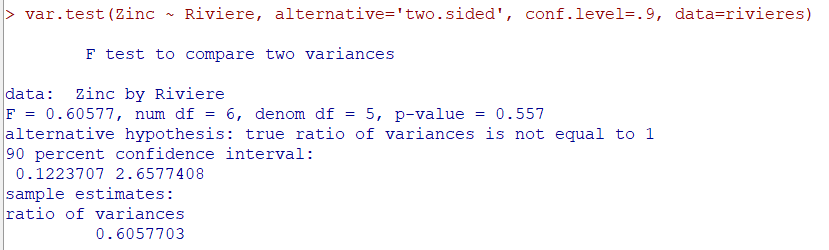
\includegraphics[width=0.85\textwidth]{images/TestF.PNG}

  \raggedright
  {
  \begin{itemize}\itemsep 1mm
    \item \texttt{F = 0.60577}, \texttt{num df = 6}, \texttt{denom df = 5} : c'est notre $F_{obs}$ et ses degrés de liberté.
    \item \texttt{p-value = 0.557} $> \alpha = 0{,}10$ \ $\Rightarrow$ on \alert{ne rejette pas} $H_0$.
    \item IC à 90\,\% pour $\sigma_1^2/\sigma_2^2$ : $[0{,}12\,;\ 2{,}66]$ \alert{contient 1} : même conclusion.
  \end{itemize}
  }
\end{frame}

\begin{frame}[plain,t]
  \centerline{\LARGE\bfseries\alert{QUIZ !}}

  \medskip
  \begin{itemize}\itemsep 0.7cm
    \item Vrai ou faux ? « Puisqu'on ne rejette pas $H_0$, on a \emph{démontré} que les deux rivières ont la même variance. »
    \item<2-> \alert{Faux.} Ne pas rejeter $H_0$ n'est pas une preuve de $H_0$ (rappel du chapitre 3c). Avec $n_1 = 7$ et $n_2 = 6$, le test $F$ a une \textbf{faible puissance} : l'IC à 90\,\% va de $0{,}12$ à $2{,}66$ !
    \item Un collègue place $s_2^2$ au numérateur : $F_{obs} = 1{,}503 / 0{,}910 = 1{,}652$. Sa conclusion change-t-elle ?
    \item<2-> \alert{Non.} Il compare à $F_{0{,}05;\,5,\,6} = 4{,}39$ : $1{,}652 < 4{,}39$, on ne rejette pas $H_0$. Même valeur-p ($0{,}557$).
  \end{itemize}
\end{frame}

\begin{frame}[t]{Attention !}
  \begin{Boite}{Le test $F$ est très sensible à la non-normalité}
    Contrairement aux tests $t$ (assez robustes), le test de Fisher peut donner des conclusions trompeuses si les populations ne sont \alert{pas normales}, même avec de grands échantillons.
  \end{Boite}

  \bigskip
  \begin{itemize}\itemsep 3mm
    \item Vérifier la normalité de \textbf{chaque} échantillon (histogramme, diagramme quantile-quantile, chapitre 2).
    \item Toujours accompagner le test d'un graphique (diagrammes en boîtes juxtaposés).
    \item Une grande différence de dispersion peut être un \alert{résultat biologique} en soi (ex. : plus grande variabilité de la réponse à un traitement).
  \end{itemize}
\end{frame}

%===============================================================================
\section{Comparaison de deux moyennes (Échantillons indépendants)}
%===============================================================================

\begin{frame}[t]{Cas 1 : Variances égales ($\sigma_1^2 = \sigma_2^2 = \sigma^2$)}
  Puisque les deux populations ont la même variance inconnue $\sigma^2$, on combine l'information des deux échantillons pour obtenir la \alert{variance combinée} (pooled variance) :

  \begin{Boite}{Variance échantillonnale combinée $S_p^2$}
    $$S_p^2 = \frac{(n_1 - 1)S_1^2 + (n_2 - 1)S_2^2}{n_1 + n_2 - 2}$$
  \end{Boite}

  \uncover<2->{
  \begin{itemize}\itemsep 1.5mm
    \item $S_p^2$ est une moyenne pondérée de $S_1^2$ et $S_2^2$ par leurs degrés de liberté.
    \item Elle possède $(n_1 - 1) + (n_2 - 1) = \alert{n_1 + n_2 - 2}$ degrés de liberté.
    \item L'erreur-type estimée de la différence des moyennes est :
      $\displaystyle \widehat{\text{ET}}(\overline{X}_1 - \overline{X}_2) = S_p\sqrt{\frac{1}{n_1} + \frac{1}{n_2}}$
  \end{itemize}
  }
\end{frame}

\begin{frame}[t]{Intervalle de confiance pour $\mu_1 - \mu_2$ (variances égales)}
  Sous l'hypothèse de normalité et de variances égales :
  \[
    T = \frac{(\overline{X}_1 - \overline{X}_2) - (\mu_1 - \mu_2)}{S_p \sqrt{\frac{1}{n_1} + \frac{1}{n_2}}} \sim t_{n_1 + n_2 - 2}
  \]

  \bigskip
  \begin{Boite}{Intervalle de confiance de niveau $1-\alpha$}
    \[
      \left[ (\overline{X}_1 - \overline{X}_2) \pm t_{n_1+n_2-2,\, \alpha/2} \, S_p \sqrt{\frac{1}{n_1} + \frac{1}{n_2}} \right]
    \]
  \end{Boite}

  \medskip
  La marge d'erreur dépend de la variance combinée $S_p^2$ et de la somme des inverses des tailles d'échantillons.
  Si l'intervalle \alert{contient 0}, on ne peut pas conclure que les moyennes diffèrent (test bilatéral au seuil $\alpha$).
\end{frame}

\begin{frame}[t]{Test d'hypothèses pour $\mu_1 - \mu_2$ (variances égales)}
  Pour tester $H_0: \mu_1 = \mu_2$ (c'est-à-dire $\mu_1 - \mu_2 = 0$) :

  \bigskip
  \begin{Boite}{Statistique observée sous $H_0$}
    \[
      t_{obs} = \frac{\overline{x}_1 - \overline{x}_2}{s_p \sqrt{\frac{1}{n_1} + \frac{1}{n_2}}}
    \]
  \end{Boite}

  \medskip
  \textbf{Règles de décision :}
  \begin{itemize}\itemsep 3mm
    \item Bilatéral ($H_1: \mu_1 \ne \mu_2$) : rejeter $H_0$ si $|t_{obs}| > t_{n_1+n_2-2,\, \alpha/2}$.
    \item Unilatéral à droite ($H_1: \mu_1 > \mu_2$) : rejeter $H_0$ si $t_{obs} > t_{n_1+n_2-2,\, \alpha}$.
    \item Unilatéral à gauche ($H_1: \mu_1 < \mu_2$) : rejeter $H_0$ si $t_{obs} < -t_{n_1+n_2-2,\, \alpha}$.
  \end{itemize}
  Ce test est souvent appelé \alert{test $t$ à deux échantillons} (\emph{two-sample t-test}).
\end{frame}

\begin{frame}[t]{Exemple 1 (suite) : Comparaison des moyennes}
  $H_0: \mu_1 = \mu_2$ contre $H_1: \mu_1 > \mu_2$ \ (question 2, $\alpha = 5\%$). \\
  Données : $n_1 = 7$, $\bar{x}_1 = 5{,}00$, $s_1^2 = 0{,}910$ ; $n_2 = 6$, $\bar{x}_2 = 4{,}39$, $s_2^2 = 1{,}503$.

  \begin{enumerate}\itemsep 1mm
    \item \textbf{Variance combinée} (le test $F$ n'a pas rejeté l'égalité) :
      $\displaystyle s_p^2 = \frac{6(0{,}910) + 5(1{,}503)}{7 + 6 - 2} = \frac{5{,}460 + 7{,}515}{11} = \mathbf{1{,}180} \implies s_p = \mathbf{1{,}086}$
    \item \textbf{Erreur-type :}
      $\widehat{\text{ET}} = 1{,}086 \sqrt{\frac{1}{7} + \frac{1}{6}} = 1{,}086 \times 0{,}5563 = \mathbf{0{,}604}$.
    \item \textbf{Statistique observée :}
      $\displaystyle t_{obs} = \frac{5{,}00 - 4{,}39}{0{,}604} = \frac{0{,}61}{0{,}604} = \mathbf{1{,}01}$
    \item<2-> \textbf{Décision :}
      avec $\nu = 7 + 6 - 2 = 11$, $t_{11;\, 0{,}05} = \mathbf{1{,}796}$.
      Puisque $t_{obs} = 1{,}01 < 1{,}796$, on \alert{ne rejette pas $H_0$} (valeur-p $= 0{,}167$).
    \item<2-> \textbf{Conclusion :} les données ne permettent pas de conclure que la concentration moyenne de zinc est plus élevée dans la rivière 1.
  \end{enumerate}
\end{frame}

\begin{frame}[t]{Exemple 1 (suite) : Région critique et valeur-p}
  \centering
  \begin{tikzpicture}
    \begin{axis}[densite, xmin=-4, xmax=4, ymax=0.45,
                 xlabel={$t$}, xtick={-4,-3,-2,-1,0,1,3,4},
                 title={Loi $t_{11}$ sous $H_0$ (test unilatéral à droite, $\alpha = 0{,}05$)}]
      \addplot[draw=none, fill=grUn!30, domain=1.01:4, samples=40] {ft(x)} \closedcycle;
      \addplot[draw=none, fill=Accent!70, domain=1.796:4, samples=30] {ft(x)} \closedcycle;
      \addplot[thick, Dominante!80!black, domain=-4:4, samples=150] {ft(x)};
      \draw[very thick, grUn] (axis cs:1.01,0) -- (axis cs:1.01,0.36)
        node[above, font=\scriptsize] {$t_{obs} = 1{,}01$};
      \node[font=\scriptsize, below] at (axis cs:1.796,0) {$1{,}796$};
      \draw[Accent!80!black, -{Stealth}] (axis cs:3.1,0.14) node[above, font=\scriptsize, align=center] {rejet\\aire $= 0{,}05$} -- (axis cs:2.3,0.03);
      \draw[grUn, -{Stealth}] (axis cs:-1.8,0.25) node[above, font=\scriptsize, align=center] {valeur-p\\aire $= 0{,}167$} -- (axis cs:1.3,0.12);
    \end{axis}
  \end{tikzpicture}

  \medskip
  \begin{itemize}\itemsep 2mm
    \item \textbf{Région critique :} $t > 1{,}796$ (zone orange).
    \item \textbf{Valeur-p :} $P(T_{11} > 1{,}01) = 0{,}167$ (zone bleue, qui \emph{contient} la zone orange) $> 0{,}05$.
  \end{itemize}
\end{frame}

\begin{frame}[t]{Exemple 1 (suite) : Sortie R de \texttt{t.test()}}
  \centering
  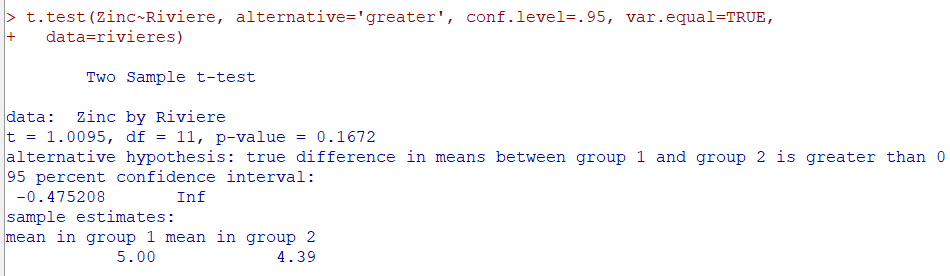
\includegraphics[width=0.92\textwidth]{images/Test-t-indep.PNG}

  \raggedright
  \small
  {
  \begin{itemize}\itemsep 1.5mm
    \item \texttt{alternative='greater'} : $H_1: \mu_1 > \mu_2$ ; \ \texttt{var.equal=TRUE} : variance combinée.
    \item \texttt{t = 1.0095}, \texttt{df = 11} : notre $t_{obs}$ (au arrondi près) et $\nu = n_1 + n_2 - 2$.
    \item \texttt{p-value = 0.1672} $> 0{,}05$ : on \alert{ne rejette pas} $H_0$.
    \item L'IC unilatéral $[-0{,}475\,;\ \infty[$ \alert{contient 0} : même conclusion.
  \end{itemize}
  }
\end{frame}

\begin{frame}[t]{Exemple 1 (suite) : Test bilatéral et intervalle de confiance}
  \textbf{À vous :} construire l'IC à 95\,\% pour $\mu_1 - \mu_2$ (utiliser $t_{11;\,0{,}025} = 2{,}201$). Vérifier ensuite avec R.

  \medskip
  \uncover<2->{
  \centering
  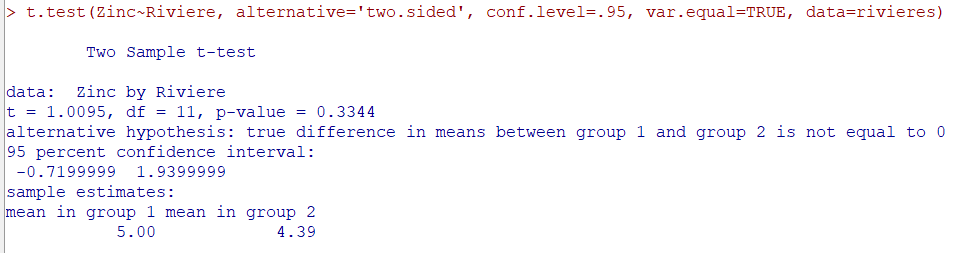
\includegraphics[width=0.92\textwidth]{images/Test-t-indep-bilat.PNG}

  \raggedright
  \small
  \begin{itemize}\itemsep 1.5mm
    \item Test bilatéral : \texttt{p-value = 0.3344} $= 2 \times 0{,}1672$ (la valeur-p bilatérale est le \alert{double} de l'unilatérale).
    \item L'IC à 95\,\% pour $\mu_1 - \mu_2$ contient 0 : pas de différence significative au seuil de 5\,\%.
  \end{itemize}
  }
\end{frame}

\begin{frame}[plain,t]
  \centerline{\LARGE\bfseries\alert{QUIZ !}}

  \medskip
  Un conseiller municipal lit le rapport et conclut : « Les deux rivières ont la même concentration moyenne de zinc. On peut choisir l'une ou l'autre. »
  \begin{itemize}\itemsep 0.9cm
    \item Êtes-vous d'accord ?
    \item<2-> \alert{Non.} « Ne pas rejeter $H_0$ » $\neq$ « $H_0$ est vraie ». L'IC à 95\,\% pour $\mu_1 - \mu_2$ va d'environ $-0{,}72$ à $1{,}94\ \mu$g/l : une différence de près de $2\ \mu$g/l reste plausible.
    \item Que faudrait-il faire pour trancher ?
    \item<2-> Augmenter les tailles d'échantillons pour gagner en \alert{puissance} (rappel 3c) et réduire la largeur de l'IC.
  \end{itemize}
\end{frame}

\begin{frame}[t]{Cas 2 : Variances inégales ($\sigma_1^2 \ne \sigma_2^2$)}
  Si le test de Fisher a rejeté l'égalité des variances, on ne peut plus utiliser $S_p^2$.
  On utilise alors l'approximation de \alert{Welch-Satterthwaite} (\alert{test de Welch}).

  \begin{Boite}{Statistique de Welch}
    $$T = \frac{(\overline{X}_1 - \overline{X}_2) - (\mu_1 - \mu_2)}{\sqrt{\frac{S_1^2}{n_1} + \frac{S_2^2}{n_2}}} \;\dot{\sim}\; t_{\nu}$$
  \end{Boite}

  \uncover<2->{
  Les degrés de liberté ajustés $\nu$ sont donnés par la formule de Welch :
  \[\nu = \frac{\left(\frac{S_1^2}{n_1} + \frac{S_2^2}{n_2}\right)^2}{\frac{(S_1^2/n_1)^2}{n_1-1} + \frac{(S_2^2/n_2)^2}{n_2-1}}\]
  En général $\nu$ n'est pas entier : avec une table, on \alert{arrondit vers le bas} (plus prudent). Dans R : \texttt{t.test(..., var.equal = FALSE)} (par défaut).
  }
\end{frame}

\begin{frame}[t]{Cas 2 : Règles de décision et intervalle de confiance}
  Sous $H_0: \mu_1 = \mu_2$, on calcule
  $\displaystyle t_{obs} = \frac{\bar{x}_1 - \bar{x}_2}{\sqrt{s_1^2/n_1 + s_2^2/n_2}}$ et :

  \begin{itemize}\itemsep 1mm
    \item Bilatéral : rejeter $H_0$ si $|t_{obs}| > t_{\nu,\, \alpha/2}$.
    \item Unilatéral à droite / à gauche : rejeter si $t_{obs} > t_{\nu,\, \alpha}$ / $t_{obs} < -t_{\nu,\, \alpha}$.
  \end{itemize}

  \begin{Boite}{IC approximatif de niveau $1-\alpha$ pour $\mu_1 - \mu_2$}
    \[
      \left[ (\bar{x}_1 - \bar{x}_2) \pm t_{\nu,\, \alpha/2} \sqrt{\frac{s_1^2}{n_1} + \frac{s_2^2}{n_2}} \right]
    \]
  \end{Boite}

  \small \alert{Remarque :} le test de Welch reste valide même si les variances sont égales (il est alors à peine moins puissant). Sur l'exemple du zinc, il donne $t_{obs} = 0{,}99$, $\nu = 9{,}42$, valeur-p $= 0{,}174$ : même conclusion.
\end{frame}

\begin{frame}[t]{Exemple 2 : Mercure dans les dorés de deux lacs}
  \small
  Des biologistes comparent la concentration de mercure (en $\mu$g/g) dans la chair de dorés jaunes pêchés dans un \textbf{réservoir hydroélectrique} récent (lac A) et dans un \textbf{lac naturel} voisin (lac B). La concentration moyenne diffère-t-elle ($\alpha = 5\%$) ?

  \smallskip
  \scriptsize
  \centering
  \begin{tabular}{lcccccccccccc}\toprule
    & \multicolumn{10}{c}{Mesures} & $\bar{x}$ & $s$ \\ \midrule
    \textbf{Lac A} ($n_1 = 8$)  & 0{,}62 & 0{,}95 & 0{,}48 & 1{,}20 & 0{,}81 & 0{,}55 & 1{,}05 & 0{,}74 & & & \textbf{0{,}800} & \textbf{0{,}2524} \\
    \textbf{Lac B} ($n_2 = 10$) & 0{,}41 & 0{,}46 & 0{,}38 & 0{,}52 & 0{,}44 & 0{,}49 & 0{,}36 & 0{,}47 & 0{,}43 & 0{,}50 & \textbf{0{,}446} & \textbf{0{,}0521} \\ \bottomrule
  \end{tabular}

  \medskip
  \begin{columns}[T]
    \column{0.45\textwidth}
      \centering
      \begin{tikzpicture}
        \begin{axis}[boites, width=5cm, height=4.3cm, xticklabels={Lac A, Lac B},
                     ylabel={Mercure ($\mu$g/g)}, ymin=0.3, ymax=1.3]
          \addplot+[boxplot prepared={median=0.775, lower quartile=0.6025,
              upper quartile=0.975, lower whisker=0.48, upper whisker=1.20},
              draw=grUn, fill=grUn!25, solid, mark=none] coordinates {};
          \addplot+[boxplot prepared={median=0.45, lower quartile=0.415,
              upper quartile=0.485, lower whisker=0.36, upper whisker=0.52},
              draw=grDeux, fill=grDeux!25, solid, mark=none] coordinates {};
        \end{axis}
      \end{tikzpicture}

    \column{0.53\textwidth}
      \small
      \begin{itemize}\itemsep 2mm
        \item<2-> Échantillons \alert{indépendants} (poissons différents, lacs différents).
        \item<2-> Les boîtes suggèrent une dispersion \alert{beaucoup plus grande} dans le lac A.
        \item<2-> Étape 1 : test $F$ ($\alpha = 10\%$). Étape 2 : test sur les moyennes.
      \end{itemize}
  \end{columns}
\end{frame}

\begin{frame}[t]{Exemple 2 (suite) : Étape 1, test de Fisher}
  $s_1^2 = 0{,}2524^2 = 0{,}06371$ \quad et \quad $s_2^2 = 0{,}0521^2 = 0{,}002716$.

  \medskip
  \begin{enumerate}\itemsep 3mm
    \item $H_0: \sigma_1^2 = \sigma_2^2$ contre $H_1: \sigma_1^2 \ne \sigma_2^2$, \ $\alpha = 0{,}10$.
    \item $\displaystyle F_{obs} = \frac{0{,}06371}{0{,}002716} = \mathbf{23{,}46}$ \quad (plus grande variance au numérateur).
    \item<2-> Valeur critique : $F_{0{,}05;\, 7,\, 9} = \mathbf{3{,}29}$.
    \item<2-> Puisque $23{,}46 > 3{,}29$, on \alert{rejette $H_0$} (valeur-p $< 0{,}0001$).
    \item<2-> \textbf{Conclusion :} la variabilité de la concentration de mercure est plus grande dans le réservoir. On \alert{ne peut pas} combiner les variances $\Rightarrow$ \textbf{test de Welch}.
  \end{enumerate}
\end{frame}

\begin{frame}[t]{Exemple 2 (suite) : Étape 2, test de Welch}
  $H_0: \mu_1 = \mu_2$ contre $H_1: \mu_1 \ne \mu_2$, \ $\alpha = 0{,}05$.

  \medskip
  \begin{enumerate}\itemsep 2mm
    \item \textbf{Erreur-type :} $\dfrac{s_1^2}{n_1} = \dfrac{0{,}06371}{8} = 0{,}007964$, \ $\dfrac{s_2^2}{n_2} = \dfrac{0{,}002716}{10} = 0{,}000272$
      $$\widehat{\text{ET}} = \sqrt{0{,}007964 + 0{,}000272} = \mathbf{0{,}0908}$$
    \item \textbf{Degrés de liberté :}
      $\displaystyle \nu = \frac{(0{,}008236)^2}{\frac{(0{,}007964)^2}{7} + \frac{(0{,}000272)^2}{9}} = \mathbf{7{,}48} \ \leadsto \ 7$
    \item \textbf{Statistique :} $\displaystyle t_{obs} = \frac{0{,}800 - 0{,}446}{0{,}0908} = \mathbf{3{,}90}$
    \item<2-> \textbf{Décision :} $|t_{obs}| = 3{,}90 > t_{7;\,0{,}025} = 2{,}365$ : on \alert{rejette $H_0$} (valeur-p $= 0{,}005$).
    \item<2-> \textbf{Conclusion :} la concentration moyenne de mercure est significativement plus élevée dans le réservoir (lac A) que dans le lac naturel.
  \end{enumerate}
\end{frame}

\begin{frame}[fragile,t]{Exemple 2 (suite) : Sortie R du test de Welch}
\begin{Verbatim}[fontsize=\scriptsize]
> A <- c(0.62, 0.95, 0.48, 1.20, 0.81, 0.55, 1.05, 0.74)
> B <- c(0.41, 0.46, 0.38, 0.52, 0.44, 0.49, 0.36, 0.47, 0.43, 0.50)
> t.test(A, B)          # var.equal = FALSE par défaut : Welch

        Welch Two Sample t-test

data:  A and B
t = 3.9008, df = 7.4787, p-value = 0.005177
alternative hypothesis: true difference in means is not equal to 0
95 percent confidence interval:
 0.1421602 0.5658398
sample estimates:
mean of x mean of y
    0.800     0.446
\end{Verbatim}

  \small
  \begin{itemize}\itemsep 1mm
    \item \texttt{df = 7.4787} : les degrés de liberté de Welch, non entiers.
    \item \textbf{À vous :} calculer l'IC à 95\,\% à la main avec $\nu = 7$ et le comparer à celui de R.
  \end{itemize}
\end{frame}

\begin{frame}[plain,t]
  \centerline{\LARGE\bfseries\alert{QUIZ !}}

  \medskip
  \begin{itemize}\itemsep 0.8cm
    \item Dans l'exemple 2, on a obtenu $\nu = 7{,}48$. Entre quelles bornes les degrés de liberté de Welch se situent-ils toujours ?
    \item<2-> $\min(n_1 - 1,\, n_2 - 1) \le \nu \le n_1 + n_2 - 2$, soit ici entre 7 et 16. Plus les variances $s_i^2/n_i$ sont déséquilibrées, plus $\nu$ est proche de la borne inférieure.
    \item Qu'aurait-on obtenu avec le test $t$ à variance combinée (à tort) ?
    \item<2-> $t_{obs} = 4{,}35$ avec 16 degrés de liberté (valeur-p $= 0{,}0005$) : un résultat \alert{trop optimiste}, car l'erreur-type est mal estimée quand les variances diffèrent autant (surtout si $n_1 \neq n_2$).
  \end{itemize}
\end{frame}

%===============================================================================
\section{Données appariées (Échantillons dépendants)}
%===============================================================================

\begin{frame}[t]{Deux scénarios d'échantillonnage}
  On veut comparer deux engrais (A et B) sur le rendement du maïs, avec 40 parcelles en tout.

  \bigskip
  \begin{Boite}{Scénario 1 : échantillons indépendants}
    20 fermes reçoivent l'engrais A, 20 \textbf{autres} fermes reçoivent l'engrais B (une parcelle par ferme).
    On note \alert{40 observations indépendantes}.
  \end{Boite}

  \pause
  \begin{Boite}{Scénario 2 : échantillons appariés}
    20 fermes : chacune est divisée en deux parcelles voisines, qui reçoivent A et B (attribution \alert{au hasard}).
    On note \alert{20 paires} d'observations.
  \end{Boite}

  \medskip
  Quel scénario permet de détecter plus facilement une différence entre les engrais ?
\end{frame}

\begin{frame}[t]{Notion d'appariement : pourquoi apparier ?}
  \begin{itemize}\itemsep 3mm
    \item \textbf{Scénario 1 :} les fermes diffèrent beaucoup (sol, climat, drainage).
      Une différence de rendement est-elle due aux \textbf{engrais} ou aux \textbf{fermes} ?
      La variance de $\overline{X}_1 - \overline{X}_2$ contient toute la \alert{variabilité entre fermes} : elle risque d'être trop grande pour conclure.
    \item \textbf{Scénario 2 :} chaque ferme sert de \alert{son propre témoin}. En comparant A et B \emph{dans} la même ferme, on élimine la variabilité entre fermes.
      Une différence significative sera due aux engrais, pourvu que l'attribution de A et B aux deux parcelles soit \alert{aléatoire}.
    \item \alert{Problème :} dans le scénario 2, $X_{1j}$ et $X_{2j}$ ne sont \textbf{pas indépendants} (même ferme).
      On ne peut pas utiliser les tests pour échantillons indépendants.
  \end{itemize}
\end{frame}

\begin{frame}[t]{Notion de données appariées}
  \begin{Boite}{Définition}
    Deux échantillons sont dits \alert{appariés} s'il existe une correspondance naturelle deux à deux entre les observations des deux groupes.
  \end{Boite}

  \textbf{Exemples typiques :}
  \begin{itemize}\itemsep 1.5mm
    \item \textbf{Mesures répétées sur le même sujet :} pression artérielle avant et après la prise d'un médicament ($X_{1i}$ et $X_{2i}$).
    \item \textbf{Paires naturelles :} les deux yeux d'un patient (un traité, l'autre témoin) ; les deux moitiés d'une feuille ; deux parcelles d'une même ferme.
    \item \textbf{Jumeaux :} l'un reçoit le traitement A, l'autre le placebo.
  \end{itemize}

  \medskip
  \uncover<2->{
    \alert{Attention :} Ne jamais appliquer un test à deux échantillons indépendants sur des données appariées (violation majeure de l'indépendance) !
  }
\end{frame}

\begin{frame}[t]{Méthode d'analyse : réduction à un échantillon}
  On calcule pour chaque paire $i$ la \alert{différence individuelle}
  $D_i = X_{1i} - X_{2i}$, \ $i = 1, \ldots, n$.
  Les $D_i$, eux, sont \alert{indépendants} d'une paire à l'autre.

  \smallskip
  Si les $D_i \sim \mathcal{N}(\mu_D, \sigma_D^2)$, le problème se ramène exactement à un \alert{test $t$ à un échantillon} (chapitre 3c) sur la moyenne des différences $\mu_D = \mu_1 - \mu_2$ !

  \medskip
  \begin{Boite}{Test $t$ apparié}
    \begin{itemize}\itemsep 1mm
      \item Moyenne des différences : $\overline{D} = \frac{1}{n}\sum_{i=1}^n D_i$
      \item Écart-type des différences : $S_D = \sqrt{\frac{1}{n-1}\sum_{i=1}^n (D_i - \overline{D})^2}$
      \item Statistique de test sous $H_0: \mu_D = 0$ :
        $\displaystyle t_{obs} = \frac{\overline{D}}{S_D / \sqrt{n}} \sim t_{n-1}$
    \end{itemize}
  \end{Boite}
\end{frame}

\begin{frame}[t]{Test apparié : règles de décision et IC}
  Pour tester $H_0: \mu_1 = \mu_2 \iff \mu_D = 0$ au seuil $\alpha$ :
  \begin{itemize}\itemsep 2mm
    \item $H_1: \mu_D \ne 0$ : rejeter $H_0$ si $|t_{obs}| > t_{n-1,\, \alpha/2}$
    \item $H_1: \mu_D > 0$ : rejeter $H_0$ si $t_{obs} > t_{n-1,\, \alpha}$
    \item $H_1: \mu_D < 0$ : rejeter $H_0$ si $t_{obs} < -t_{n-1,\, \alpha}$
  \end{itemize}

  \bigskip
  \begin{Boite}{Intervalle de confiance de niveau $1-\alpha$ pour $\mu_D$}
    \[
      \left[ \overline{D} \pm t_{n-1,\, \alpha/2} \, \frac{S_D}{\sqrt{n}} \right]
    \]
  \end{Boite}

  \medskip
  \alert{Attention :} $n$ est le nombre de \textbf{paires}, pas le nombre total de mesures.
\end{frame}

\begin{frame}[t]{Exemple 3 : Un antihypertenseur}
  \small
  On mesure la pression artérielle systolique (mmHg) de 10 patients hypertendus \textbf{avant} et \textbf{après} 8 semaines de traitement. Le médicament diminue-t-il la pression moyenne ($\alpha = 5\%$) ?

  \smallskip
  \centering
  \scriptsize
  \begin{tabular}{lccccccccccc}\toprule
    \textbf{Patient} & 1 & 2 & 3 & 4 & 5 & 6 & 7 & 8 & 9 & 10 & Moy. \\ \midrule
    Avant ($x_{1i}$)       & 152 & 138 & 165 & 147 & 171 & 143 & 158 & 136 & 161 & 149 & 152{,}0 \\
    Après ($x_{2i}$)       & 141 & 133 & 154 & 140 & 160 & 139 & 146 & 131 & 155 & 138 & 143{,}7 \\ \midrule
    \uncover<2->{$d_i = x_{1i} - x_{2i}$} & \uncover<2->{11} & \uncover<2->{5} & \uncover<2->{11} & \uncover<2->{7} & \uncover<2->{11} & \uncover<2->{4} & \uncover<2->{12} & \uncover<2->{5} & \uncover<2->{6} & \uncover<2->{11} & \uncover<2->{\textbf{8{,}3}} \\ \bottomrule
  \end{tabular}

  \medskip
  \raggedright
  \small
  \begin{itemize}\itemsep 2mm
    \item<2-> Données \alert{appariées} : les deux mesures proviennent du \textbf{même patient}.
    \item<2-> $H_0: \mu_D = 0$ contre $H_1: \mu_D > 0$ (la pression \emph{baisse} : avant $>$ après).
    \item<2-> Écarts-types : $s_{\text{avant}} = 11{,}6$, \ $s_{\text{après}} = 9{,}8$, mais \ $s_D = \mathbf{3{,}16}$ seulement !
  \end{itemize}
\end{frame}

\begin{frame}[t]{Exemple 3 (suite) : L'appariement en image}
  \centering
  \begin{tikzpicture}
    \begin{axis}[boites, width=5.3cm, height=5.2cm, xticklabels={Avant, Après},
                 ylabel={PAS (mmHg)}, ymin=128, ymax=175,
                 yticklabel style={/pgf/number format/precision=0},
                 title={Vue « indépendante »}]
      \addplot+[boxplot prepared={median=150.5, lower quartile=144,
          upper quartile=160.25, lower whisker=136, upper whisker=171},
          draw=grUn, fill=grUn!25, solid, mark=none] coordinates {};
      \addplot+[boxplot prepared={median=140.5, lower quartile=138.25,
          upper quartile=152, lower whisker=131, upper whisker=160},
          draw=grDeux, fill=grDeux!25, solid, mark=none] coordinates {};
    \end{axis}
  \end{tikzpicture}
  \hfill
  \begin{tikzpicture}
    \begin{axis}[boites, width=5.3cm, height=5.2cm, xticklabels={Avant, Après},
                 ymin=128, ymax=175, ymajorgrids,
                 yticklabel style={/pgf/number format/precision=0},
                 title={Vue « appariée »},
                 paire/.style={mark=*, mark size=1.2pt, black!55, thin}]
      \addplot[paire] coordinates {(1,152) (2,141)};
      \addplot[paire] coordinates {(1,138) (2,133)};
      \addplot[paire] coordinates {(1,165) (2,154)};
      \addplot[paire] coordinates {(1,147) (2,140)};
      \addplot[paire] coordinates {(1,171) (2,160)};
      \addplot[paire] coordinates {(1,143) (2,139)};
      \addplot[paire] coordinates {(1,158) (2,146)};
      \addplot[paire] coordinates {(1,136) (2,131)};
      \addplot[paire] coordinates {(1,161) (2,155)};
      \addplot[paire] coordinates {(1,149) (2,138)};
    \end{axis}
  \end{tikzpicture}

  \small
  \raggedright
  \begin{itemize}\itemsep 1mm
    \item À gauche, les boîtes se chevauchent : la \alert{variabilité entre patients} masque l'effet.
    \item À droite, \alert{les 10 segments descendent} : chaque patient baisse, de 4 à 12 mmHg.
  \end{itemize}
\end{frame}

\begin{frame}[t]{Exemple 3 (suite) : Solution}
  $n = 10$ paires, \ $\bar{d} = 8{,}3$ mmHg, \ $s_D = 3{,}164$ mmHg.

  \medskip
  \begin{enumerate}\itemsep 3mm
    \item \textbf{Erreur-type :} $s_D / \sqrt{n} = 3{,}164 / \sqrt{10} = \mathbf{1{,}001}$.
    \item \textbf{Statistique observée :}
      $\displaystyle t_{obs} = \frac{\bar{d}}{s_D/\sqrt{n}} = \frac{8{,}3}{1{,}001} = \mathbf{8{,}30}$
    \item<2-> \textbf{Décision :} $t_{9;\,0{,}05} = 1{,}833$. Puisque $8{,}30 > 1{,}833$, on \alert{rejette $H_0$} (valeur-p $< 0{,}0001$).
    \item<2-> \textbf{Conclusion :} le traitement diminue significativement la pression artérielle systolique moyenne des patients.
    \item<2-> \textbf{À vous :} calculer l'IC à 95\,\% pour $\mu_D$ (utiliser $t_{9;\,0{,}025} = 2{,}262$) et l'interpréter.
  \end{enumerate}

  \medskip
  \uncover<2->{
  \small Dans R : \texttt{t.test(avant, apres, paired = TRUE, alternative = "greater")} donne \texttt{t = 8.2954, df = 9, p-value = 8.274e-06}.
  }
\end{frame}

\begin{frame}[plain,t]
  \centerline{\LARGE\bfseries\alert{QUIZ !}}

  \medskip
  Par erreur, vous analysez l'exemple 3 comme s'il s'agissait d'échantillons \emph{indépendants} avec variances égales ($\alpha = 5\%$, $H_1: \mu_1 > \mu_2$).
  \begin{itemize}\itemsep 0.6cm
    \item Quelle est votre règle de rejet de $H_0$ ?
    \item<2-> $\nu = 10 + 10 - 2 = 18$ : rejeter $H_0$ si $t_{obs} > t_{18;\,0{,}05} = 1{,}734$.
    \item On obtient $s_p = 10{,}72$ et $t_{obs} = 8{,}3 / (10{,}72\sqrt{2/10}) = 1{,}73$. Conclusion ?
    \item<2-> $1{,}73 < 1{,}734$ : on \alert{ne rejetterait pas} $H_0$ (valeur-p $= 0{,}050$) ! L'erreur-type ($4{,}80$ au lieu de $1{,}00$) inclut la variabilité entre patients. \alert{Ignorer l'appariement fait perdre beaucoup de puissance.}
  \end{itemize}
\end{frame}

\begin{frame}[t]{Lecture d'une sortie R : zinc au fond et en surface}
  \small
  On mesure la concentration de zinc \textbf{au fond} et \textbf{en surface} de l'eau à 6 sites d'un lac (deux mesures \alert{au même site}).
  L'eau du fond est-elle plus chargée en zinc ($\alpha = 1\%$) ?

  \smallskip
  \centering
  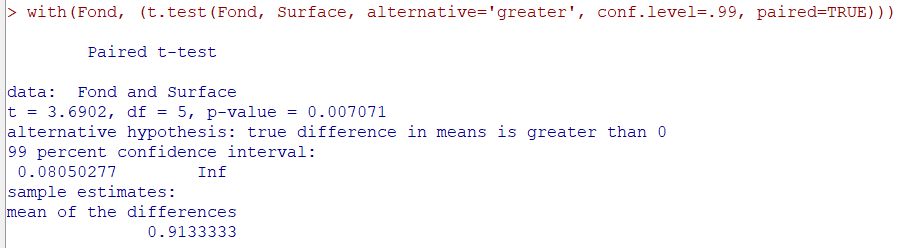
\includegraphics[width=0.9\textwidth]{images/Test-t-pair.PNG}

  \raggedright
  {
  \begin{itemize}\itemsep 1mm
    \item \texttt{paired=TRUE} : test $t$ sur les 6 différences $d_i = \text{fond}_i - \text{surface}_i$ ; \texttt{df = 5} $= n - 1$.
    \item $\bar{d} = 0{,}913$ ; $t_{obs} = 3{,}69$ ; \texttt{p-value = 0.007} $< 0{,}01$ $\Rightarrow$ on \alert{rejette $H_0$}.
    \item Au seuil de 1\,\%, la concentration moyenne est plus élevée au fond qu'en surface.
  \end{itemize}
  }
\end{frame}

\begin{frame}[t]{Quelques remarques importantes}
  \begin{itemize}\itemsep 5mm
    \item C'est le \alert{contexte} (le plan d'expérience) qui détermine si les données sont appariées ou non, pas les nombres eux-mêmes.
    \item Si on analyse des données appariées \alert{sans tenir compte de l'appariement}, on risque de diminuer grandement la significativité des données (valeur-p surestimée), comme dans le quiz précédent.
    \item L'appariement est avantageux quand les \alert{unités expérimentales sont hétérogènes} (patients, fermes, sites) : on retire la variabilité entre unités.
    \item Pour des mesures « avant/après », prudence : sans groupe témoin, un autre facteur (saison, effet placebo) peut expliquer le changement.
  \end{itemize}
\end{frame}

\begin{frame}[plain,t]
  \centerline{\LARGE\bfseries\alert{QUIZ !}}

  \medskip
  Appariés ou indépendants ?
  \small
  \begin{enumerate}\itemsep 2.5mm
    \item On mesure la glycémie de 15 patients avec deux glucomètres différents (chaque patient est mesuré avec les deux appareils). \\
      \uncover<2->{$\Rightarrow$ \alert{Appariés} (même patient).}
    \item On compare la masse de 12 souris nourries au régime A à celle de 12 autres souris nourries au régime B. \\
      \uncover<2->{$\Rightarrow$ \alert{Indépendants} (souris différentes, aucune correspondance).}
    \item On compte les stomates sur la face supérieure et la face inférieure de 20 feuilles. \\
      \uncover<2->{$\Rightarrow$ \alert{Appariés} (les deux faces d'une même feuille).}
    \item On compare l'abondance d'une espèce d'insecte dans 8 champs biologiques et 8 champs conventionnels. \\
      \uncover<2->{$\Rightarrow$ \alert{Indépendants}, sauf si les champs sont formés en paires voisines (même sol).}
  \end{enumerate}
\end{frame}

%===============================================================================
\section{Comparaison de deux proportions}
%===============================================================================

\begin{frame}[t]{Comparaison de deux proportions}
  Soient deux échantillons indépendants de grandes tailles :
  $Y_1 \sim \text{Binomiale}(n_1, p_1)$ et $Y_2 \sim \text{Binomiale}(n_2, p_2)$.

  \smallskip
  Estimations ponctuelles : $\hat{p}_1 = Y_1/n_1$ et $\hat{p}_2 = Y_2/n_2$.

  \medskip
  \begin{Boite}{Test d'hypothèses d'égalité des proportions}
    On estime la proportion commune sous $H_0: p_1 = p_2$ par la \alert{proportion combinée}
    $\displaystyle \widehat{P} = \frac{Y_1 + Y_2}{n_1 + n_2}$.

    \smallskip
    Statistique de test (normale centrée réduite) :
    \[
      Z = \frac{\hat{p}_1 - \hat{p}_2}{\sqrt{\widehat{P}(1 - \widehat{P})\left(\frac{1}{n_1} + \frac{1}{n_2}\right)}} \;\dot{\sim}\; \mathcal{N}(0, 1)
    \]
  \end{Boite}
\end{frame}

\begin{frame}[t]{Règles de décision, conditions et intervalle de confiance}
  \begin{itemize}\itemsep 1.5mm
    \item Bilatéral : rejeter $H_0$ si $|z_{obs}| > z_{\alpha/2}$ ; \ unilatéral : $z_{obs} > z_\alpha$ ou $z_{obs} < -z_\alpha$.
    \item \textbf{Conditions} (approximation normale) : $n_i \widehat{P} \ge 5$ et $n_i(1 - \widehat{P}) \ge 5$ pour $i = 1, 2$.
  \end{itemize}

  \begin{Boite}{Intervalle de confiance de niveau $1-\alpha$ pour $p_1 - p_2$}
    \[
      \left[ (\hat{p}_1 - \hat{p}_2) \pm z_{\alpha/2} \sqrt{\frac{\hat{p}_1(1-\hat{p}_1)}{n_1} + \frac{\hat{p}_2(1-\hat{p}_2)}{n_2}} \right]
    \]
  \end{Boite}

  \pause
  \alert{Attention :} l'erreur-type n'est pas la même !
  \begin{itemize}\itemsep 1.5mm
    \item Pour le \textbf{test}, on se place sous $H_0$ ($p_1 = p_2$) : on utilise $\widehat{P}$ combinée.
    \item Pour l'\textbf{IC}, on ne suppose pas $p_1 = p_2$ : on utilise $\hat{p}_1$ et $\hat{p}_2$ séparément.
  \end{itemize}
\end{frame}

\begin{frame}[t]{Exemple 4 : Taux de guérison de deux traitements}
  Un essai clinique randomisé compare un \textbf{nouvel antibiotique} au \textbf{traitement standard} contre une infection urinaire. Guérison après 14 jours :

  \medskip
  \centering
  \small
  \begin{tabular}{lccc}\toprule
    & Patients ($n_i$) & Guéris ($y_i$) & $\hat{p}_i$ \\ \midrule
    Nouvel antibiotique (1) & 120 & 90 & $0{,}750$ \\
    Traitement standard (2) & 110 & 66 & $0{,}600$ \\ \bottomrule
  \end{tabular}

  \raggedright
  \bigskip
  Au seuil $\alpha = 5\%$, les taux de guérison diffèrent-ils ?

  \medskip
  \begin{itemize}\itemsep 2mm
    \item<2-> Deux groupes de patients \alert{différents} (attribution au hasard) : échantillons indépendants.
    \item<2-> $H_0: p_1 = p_2$ contre $H_1: p_1 \ne p_2$.
    \item<2-> $\widehat{P} = \dfrac{90 + 66}{120 + 110} = \dfrac{156}{230} = \mathbf{0{,}678}$ ;
      conditions : $n_1\widehat{P} = 81{,}4$, $n_1(1-\widehat{P}) = 38{,}6$, $n_2\widehat{P} = 74{,}6$, $n_2(1-\widehat{P}) = 35{,}4$, tous $\ge 5$.
  \end{itemize}
\end{frame}

\begin{frame}[t]{Exemple 4 (suite) : Solution}
  \begin{enumerate}\itemsep 1.5mm
    \item \textbf{Erreur-type sous $H_0$ :}
      $\sqrt{0{,}678 \times 0{,}322 \left(\frac{1}{120} + \frac{1}{110}\right)} = \sqrt{0{,}2182 \times 0{,}01742} = \mathbf{0{,}0617}$
    \item \textbf{Statistique observée :}
      $\displaystyle z_{obs} = \frac{0{,}750 - 0{,}600}{0{,}0617} = \mathbf{2{,}43}$
    \item \textbf{Décision :} $|z_{obs}| = 2{,}43 > z_{0{,}025} = 1{,}96$ : on \alert{rejette $H_0$}. Valeur-p $= 2\,P(Z > 2{,}43) = 0{,}015$.
    \item<2-> \textbf{IC à 95\,\% pour $p_1 - p_2$ :}
      $\widehat{\text{ET}} = \sqrt{\frac{0{,}75 \times 0{,}25}{120} + \frac{0{,}60 \times 0{,}40}{110}} = 0{,}0612$
      \\ $0{,}150 \pm 1{,}96 \times 0{,}0612 = 0{,}150 \pm 0{,}120 = [\mathbf{0{,}030}\,;\ \mathbf{0{,}270}]$
    \item<2-> \textbf{Conclusion :} le nouvel antibiotique a un taux de guérison significativement plus élevé : de 3 à 27 points de pourcentage de plus que le traitement standard (confiance 95\,\%).
  \end{enumerate}
\end{frame}

\begin{frame}[t]{Exemple 4 (suite) : La décision en image}
  \centering
  \begin{tikzpicture}
    \begin{axis}[densite, xmin=-3.8, xmax=3.8, ymax=0.45,
                 xlabel={$z$}, xtick={-3,-1,0,1,3},
                 title={Loi $\mathcal{N}(0,1)$ sous $H_0$ (test bilatéral, $\alpha = 0{,}05$)}]
      \addplot[draw=none, fill=Accent!60, domain=-3.8:-1.96, samples=30] {fz(x)} \closedcycle;
      \addplot[draw=none, fill=Accent!60, domain=1.96:3.8, samples=30] {fz(x)} \closedcycle;
      \addplot[thick, Dominante!80!black, domain=-3.8:3.8, samples=150] {fz(x)};
      \draw[very thick, grUn] (axis cs:2.43,0) -- (axis cs:2.43,0.2)
        node[above, font=\scriptsize] {$z_{obs} = 2{,}43$};
      \node[font=\scriptsize, below] at (axis cs:-1.96,0) {$-1{,}96$};
      \node[font=\scriptsize, below] at (axis cs:1.96,0) {$1{,}96$};
      \node[font=\scriptsize, Accent!80!black] at (axis cs:-3,0.1) {$0{,}025$};
      \node[font=\scriptsize, Accent!80!black] at (axis cs:3.2,0.1) {$0{,}025$};
    \end{axis}
  \end{tikzpicture}

  \medskip
  \begin{itemize}\itemsep 2mm
    \item $z_{obs}$ tombe dans la \alert{région critique} : on rejette $H_0$.
    \item Cohérent avec l'IC à 95\,\% $[0{,}030\,;\ 0{,}270]$, qui \alert{ne contient pas 0}.
  \end{itemize}
\end{frame}

\begin{frame}[fragile,t]{Exemple 4 (suite) : Sortie R de \texttt{prop.test()}}
\begin{Verbatim}[fontsize=\scriptsize]
> prop.test(x = c(90, 66), n = c(120, 110), correct = FALSE)

        2-sample test for equality of proportions without continuity correction

data:  c(90, 66) out of c(120, 110)
X-squared = 5.9174, df = 1, p-value = 0.01499
alternative hypothesis: two.sided
95 percent confidence interval:
 0.03006817 0.26993183
sample estimates:
prop 1 prop 2
  0.75   0.60
\end{Verbatim}

  \small
  \begin{itemize}\itemsep 1.5mm
    \item R affiche $X^2 = z_{obs}^2$ : $2{,}433^2 = 5{,}917$ (un khi-deux à 1 d.l., voir chapitre 7). Même valeur-p : $0{,}015$.
    \item \texttt{correct = FALSE} : sans correction de continuité, pour retrouver le test $z$ du cours (par défaut, R applique une correction).
    \item L'IC est exactement celui calculé à la main.
  \end{itemize}
\end{frame}

\begin{frame}[plain,t]
  \centerline{\LARGE\bfseries\alert{QUIZ !}}

  \medskip
  Une petite étude pilote avait obtenu les \emph{mêmes proportions} : 9 guéris sur 12 (nouvel antibiotique) et 6 sur 10 (standard).
  \begin{itemize}\itemsep 0.7cm
    \item La différence observée ($0{,}15$) est la même. La conclusion est-elle la même ?
    \item<2-> \alert{Non.} $\widehat{P} = 15/22 = 0{,}682$, erreur-type $= 0{,}199$, $z_{obs} = 0{,}75$ (valeur-p $= 0{,}45$) : on ne rejette pas $H_0$. La même différence n'est pas significative avec de petits échantillons.
    \item Le test est-il seulement valide ici ?
    \item<2-> Douteux : $n_2(1 - \widehat{P}) = 10 \times 0{,}318 = 3{,}2 < 5$. R avertit d'ailleurs : \texttt{Chi-squared approximation may be incorrect}.
  \end{itemize}
\end{frame}

%===============================================================================
\section{Synthèse : choisir le bon test}
%===============================================================================

\begin{frame}[t]{Quel test utiliser ?}
  \centering
  \ArbreDecision
\end{frame}

\begin{frame}[plain,t]
  \centerline{\LARGE\bfseries\alert{QUIZ !}}

  \medskip
  Quel test utiliser ?
  \small
  \begin{enumerate}\itemsep 3mm
    \item La variabilité du calibre des pommes diffère-t-elle entre deux vergers ? \uncover<2->{$\Rightarrow$ \alert{Test $F$ de Fisher} (\texttt{var.test}).}
    \item Proportion de tiques porteuses de la bactérie de la maladie de Lyme dans deux régions ($n = 250$ et $300$ tiques). \uncover<2->{$\Rightarrow$ \alert{Test $z$ pour deux proportions} (\texttt{prop.test}).}
    \item Masse de souris de deux lignées ($n = 12$ et $15$) ; le test $F$ rejette l'égalité des variances. \uncover<2->{$\Rightarrow$ \alert{Test de Welch} (\texttt{t.test}, \texttt{var.equal = FALSE}).}
    \item Fréquence cardiaque au repos de 20 athlètes avant et après un programme d'entraînement. \uncover<2->{$\Rightarrow$ \alert{Test $t$ apparié} (\texttt{paired = TRUE}).}
    \item Longueur de truites de deux lacs ($n = 25$ chacun) ; le test $F$ ne rejette pas l'égalité des variances. \uncover<2->{$\Rightarrow$ \alert{Test $t$ à variance combinée} (\texttt{var.equal = TRUE}).}
  \end{enumerate}
\end{frame}

\begin{frame}[t]{Tableau récapitulatif du Chapitre 4}
  \centering
  \scriptsize
  \renewcommand{\arraystretch}{1.3}
  \begin{tabular}{lll}\toprule
    \textbf{Problème} & \textbf{Statistique de test} & \textbf{Loi sous $H_0$} \\ \midrule
    $H_0: \sigma_1^2 = \sigma_2^2$ (indép.) & $F_{obs} = \frac{S_1^2}{S_2^2}$ & $\mathcal{F}(n_1-1,\, n_2-1)$ \\[2mm]
    $H_0: \mu_1 = \mu_2$ ($\sigma^2$ égales) & $t_{obs} = \frac{\overline{X}_1 - \overline{X}_2}{S_p \sqrt{1/n_1 + 1/n_2}}$ & $t_{n_1+n_2-2}$ \\[2mm]
    $H_0: \mu_1 = \mu_2$ ($\sigma^2$ inégales) & $t_{obs} = \frac{\overline{X}_1 - \overline{X}_2}{\sqrt{S_1^2/n_1 + S_2^2/n_2}}$ & $t_\nu$ (Welch) \\[2mm]
    $H_0: \mu_1 = \mu_2$ (appariés) & $t_{obs} = \frac{\overline{D}}{S_D / \sqrt{n}}$ & $t_{n-1}$ \\[2mm]
    $H_0: p_1 = p_2$ (grandes tailles) & $z_{obs} = \frac{\hat{p}_1 - \hat{p}_2}{\sqrt{\widehat{P}(1-\widehat{P})(1/n_1 + 1/n_2)}}$ & $\mathcal{N}(0, 1)$ \\ \bottomrule
  \end{tabular}

  \bigskip
  \normalsize
  Tous ces tests sont disponibles sous R avec \texttt{var.test()}, \texttt{t.test()} et \texttt{prop.test()}.
\end{frame}

\begin{frame}[t]{Réponses aux exemples}
  \footnotesize
  \begin{enumerate}\itemsep 1.5mm
    \item[1.] \textbf{Zinc.} Test $F$ : $0{,}228 \le F_{obs} = 0{,}606 \le 4{,}95$ (valeur-p $= 0{,}557$), on ne rejette pas l'égalité des variances.
      Test $t$ ($H_1: \mu_1 > \mu_2$) : $t_{obs} = 1{,}01 < 1{,}796$ (valeur-p $= 0{,}167$), on ne rejette pas $H_0$ : la concentration moyenne de la rivière 1 n'excède pas celle de la rivière 2 de façon significative.
      IC à 95\,\% pour $\mu_1 - \mu_2$ : $0{,}61 \pm 2{,}201 \times 0{,}604 = [-0{,}72\,;\ 1{,}94]\ \mu$g/l.
    \item[2.] \textbf{Mercure.} $F_{obs} = 23{,}46 > 3{,}29$ : variances inégales. Welch : $t_{obs} = 3{,}90$, $\nu = 7{,}48$, $|t_{obs}| > 2{,}365$ (valeur-p $= 0{,}005$), on rejette $H_0$.
      IC à 95\,\% avec $\nu = 7$ : $0{,}354 \pm 2{,}365 \times 0{,}0908 = [0{,}139\,;\ 0{,}569]\ \mu$g/g (R, avec $\nu = 7{,}48$ : $[0{,}142\,;\ 0{,}566]$).
    \item[3.] \textbf{Antihypertenseur.} $t_{obs} = 8{,}30 > 1{,}833$ (valeur-p $< 0{,}0001$), on rejette $H_0$.
      IC à 95\,\% pour $\mu_D$ : $8{,}3 \pm 2{,}262 \times 1{,}001 = [6{,}04\,;\ 10{,}56]$ mmHg : baisse moyenne entre 6 et 10,6 mmHg.
      Analyse (erronée) en échantillons indépendants : $t_{obs} = 1{,}73 < 1{,}734$, valeur-p $= 0{,}050$.
    \item[4.] \textbf{Guérison.} $z_{obs} = 2{,}43 > 1{,}96$ (valeur-p $= 0{,}015$), on rejette $H_0$ ; IC à 95\,\% pour $p_1 - p_2$ : $[0{,}030\,;\ 0{,}270]$.
      Étude pilote : $z_{obs} = 0{,}75$ (valeur-p $= 0{,}45$), conditions non respectées.
    \item[5.] \textbf{Zinc fond/surface} (sortie R) : $t_{obs} = 3{,}69$, 5 d.l., valeur-p $= 0{,}007 < 0{,}01$ : on rejette $H_0$.
  \end{enumerate}
\end{frame}

\end{document}
